
\documentclass{article}
\usepackage[spanish]{babel} %Definir idioma español
\usepackage[utf8]{inputenc} %Codificacion utf-8
\usepackage{amssymb, amsmath, amsbsy, wasysym}
\usepackage{multirow} % para tablas
\usepackage{graphicx}
\usepackage[ruled, vlined, spanish, linesnumbered]{algorithm2e} %Para escribir algoritmos
\title{Tarea 3\\Programación avanzada}
\author{Emmanuel Peto Gutiérrez}
\begin{document}
\maketitle

\section{Ejercicio arreglo}

Primero se explicará qué pasa cuando se igualan los arreglos. Esto es\\
\texttt{int[] arregloDos = arregloUno;}

Cuando se ejecuta el comando \texttt{new int[3]} se está creando un arreglo, el cual llamaré \textit{nai3} (aunque en realidad no tiene nombre), y se guarda en alguna dirección en la memoria. Del lado izquierdo del comando \texttt{int[] arregloUno = new int[3]}, se observa que se está declarando un arreglo llamado \texttt{arregloUno}, el cual apunta a \textit{nai3}. Al hacer \texttt{arregloDos = arregloUno} lo que ocurre es que \texttt{arregloDos} está apuntando a \textit{nai3}; es decir, \texttt{arregloUno} y \texttt{arregloDos} apuntan al mismo arreglo. Al modificar cualquier variable, \texttt{arregloUno} o \texttt{arregloDos}, en realidad se está modificando al arreglo \textit{nai3}, por lo cual, al imprimir cualquiera de los dos se muestra lo mismo, aunque sólo se haya modificado uno.

Ahora se explicará el caso en el que se copia \texttt{arregloUno}. Es decir, en la línea:\\
\texttt{int[] arregloTres = arregloUno.clone();}

Lo que ocurre dentro del método \texttt{clone()} es que se crea un arreglo nuevo, se copia cada elemento de \texttt{arregloUno} al nuevo y finalmente se devuelve el nuevo. El identificador \texttt{arregloTres} apunta al nuevo arreglo, que es una clon del arreglo apuntado por \texttt{arregloUno} pero no es el mismo (están en diferentes direcciones de memoria).

\section{Ejercicio heap}

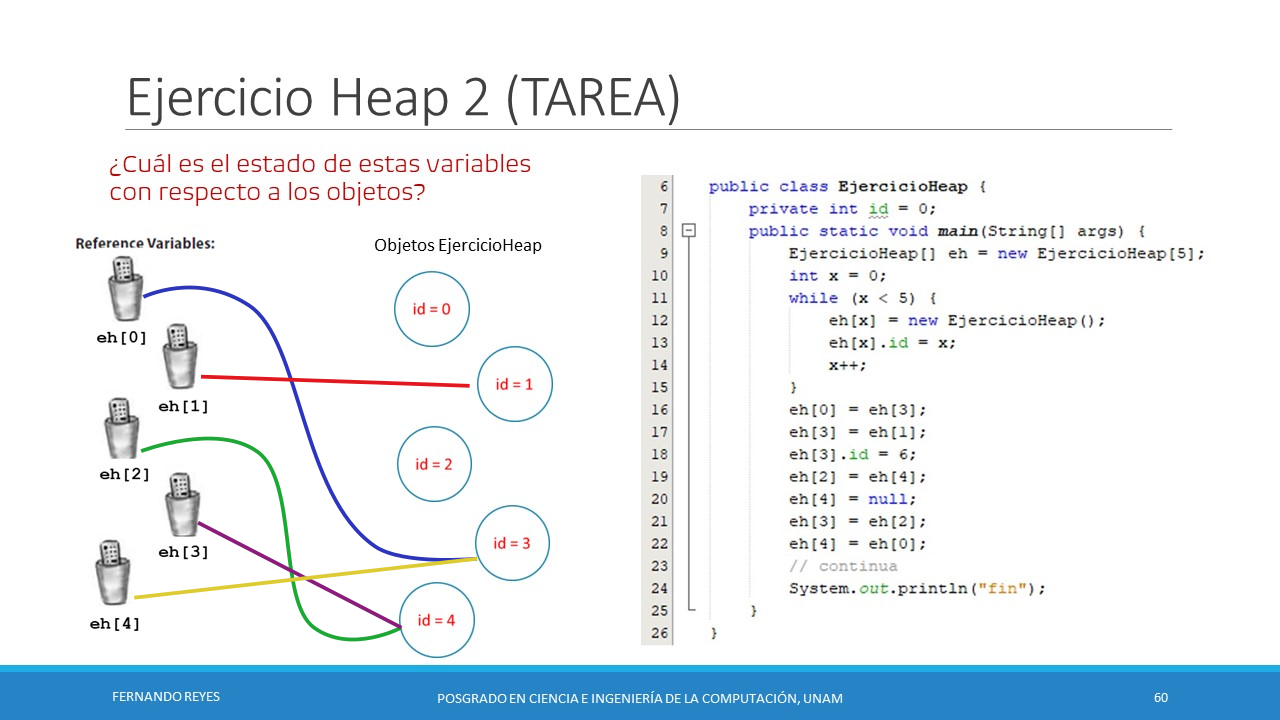
\includegraphics[width=\linewidth]{ejercicioheap2.png}

El objeto que inicialmente tenía \textit{id} 1, al final tiene \textit{id} 6.

\end{document}

